Graph Convolutional Networks (GCNs) \cite{gcn} are an efficient variant of Convolutional Neural Networks (CNNs) on graphs. 
GCNs stack layers of learned first-order spectral filters followed by a nonlinear activation function to learn graph representations.
Recently, GCNs and subsequent variants have achieved state-of-the-art results in various application areas, including but not limited to citation networks \cite{gcn}, social networks \cite{FastGCN}, applied chemistry \cite{liao2018lanczosnet}, natural language processing \cite{textGCN, han2012geolocation, relation-extraction}, and computer vision \cite{wang2018zero, ADGPM}.  

Historically, the development of machine learning algorithms has followed a clear trend from initial simplicity to need-driven complexity. For instance, limitations of the linear Perceptron \cite{rosenblatt1958perceptron} motivated the development of the more complex but also more expressive neural network (or multi-layer Perceptrons, MLPs)~\cite{rosenblatt1961principles}. Similarly, simple pre-defined linear image filters~\cite{sobel19683x3,harris1988combined} eventually gave rise to nonlinear CNNs with learned convolutional kernels ~\cite{waibel1989phoneme,lecun1989backpropagation}. 
As additional algorithmic complexity tends to complicate theoretical analysis and obfuscates understanding, it is typically only introduced  for applications where simpler methods are insufficient.  Arguably, most classifiers in real world applications are still linear (typically logistic regression), which are straight-forward to optimize and easy to interpret. 

% \input{figures/progress.tex}

\begin{figure*}[h!]
    \centering
    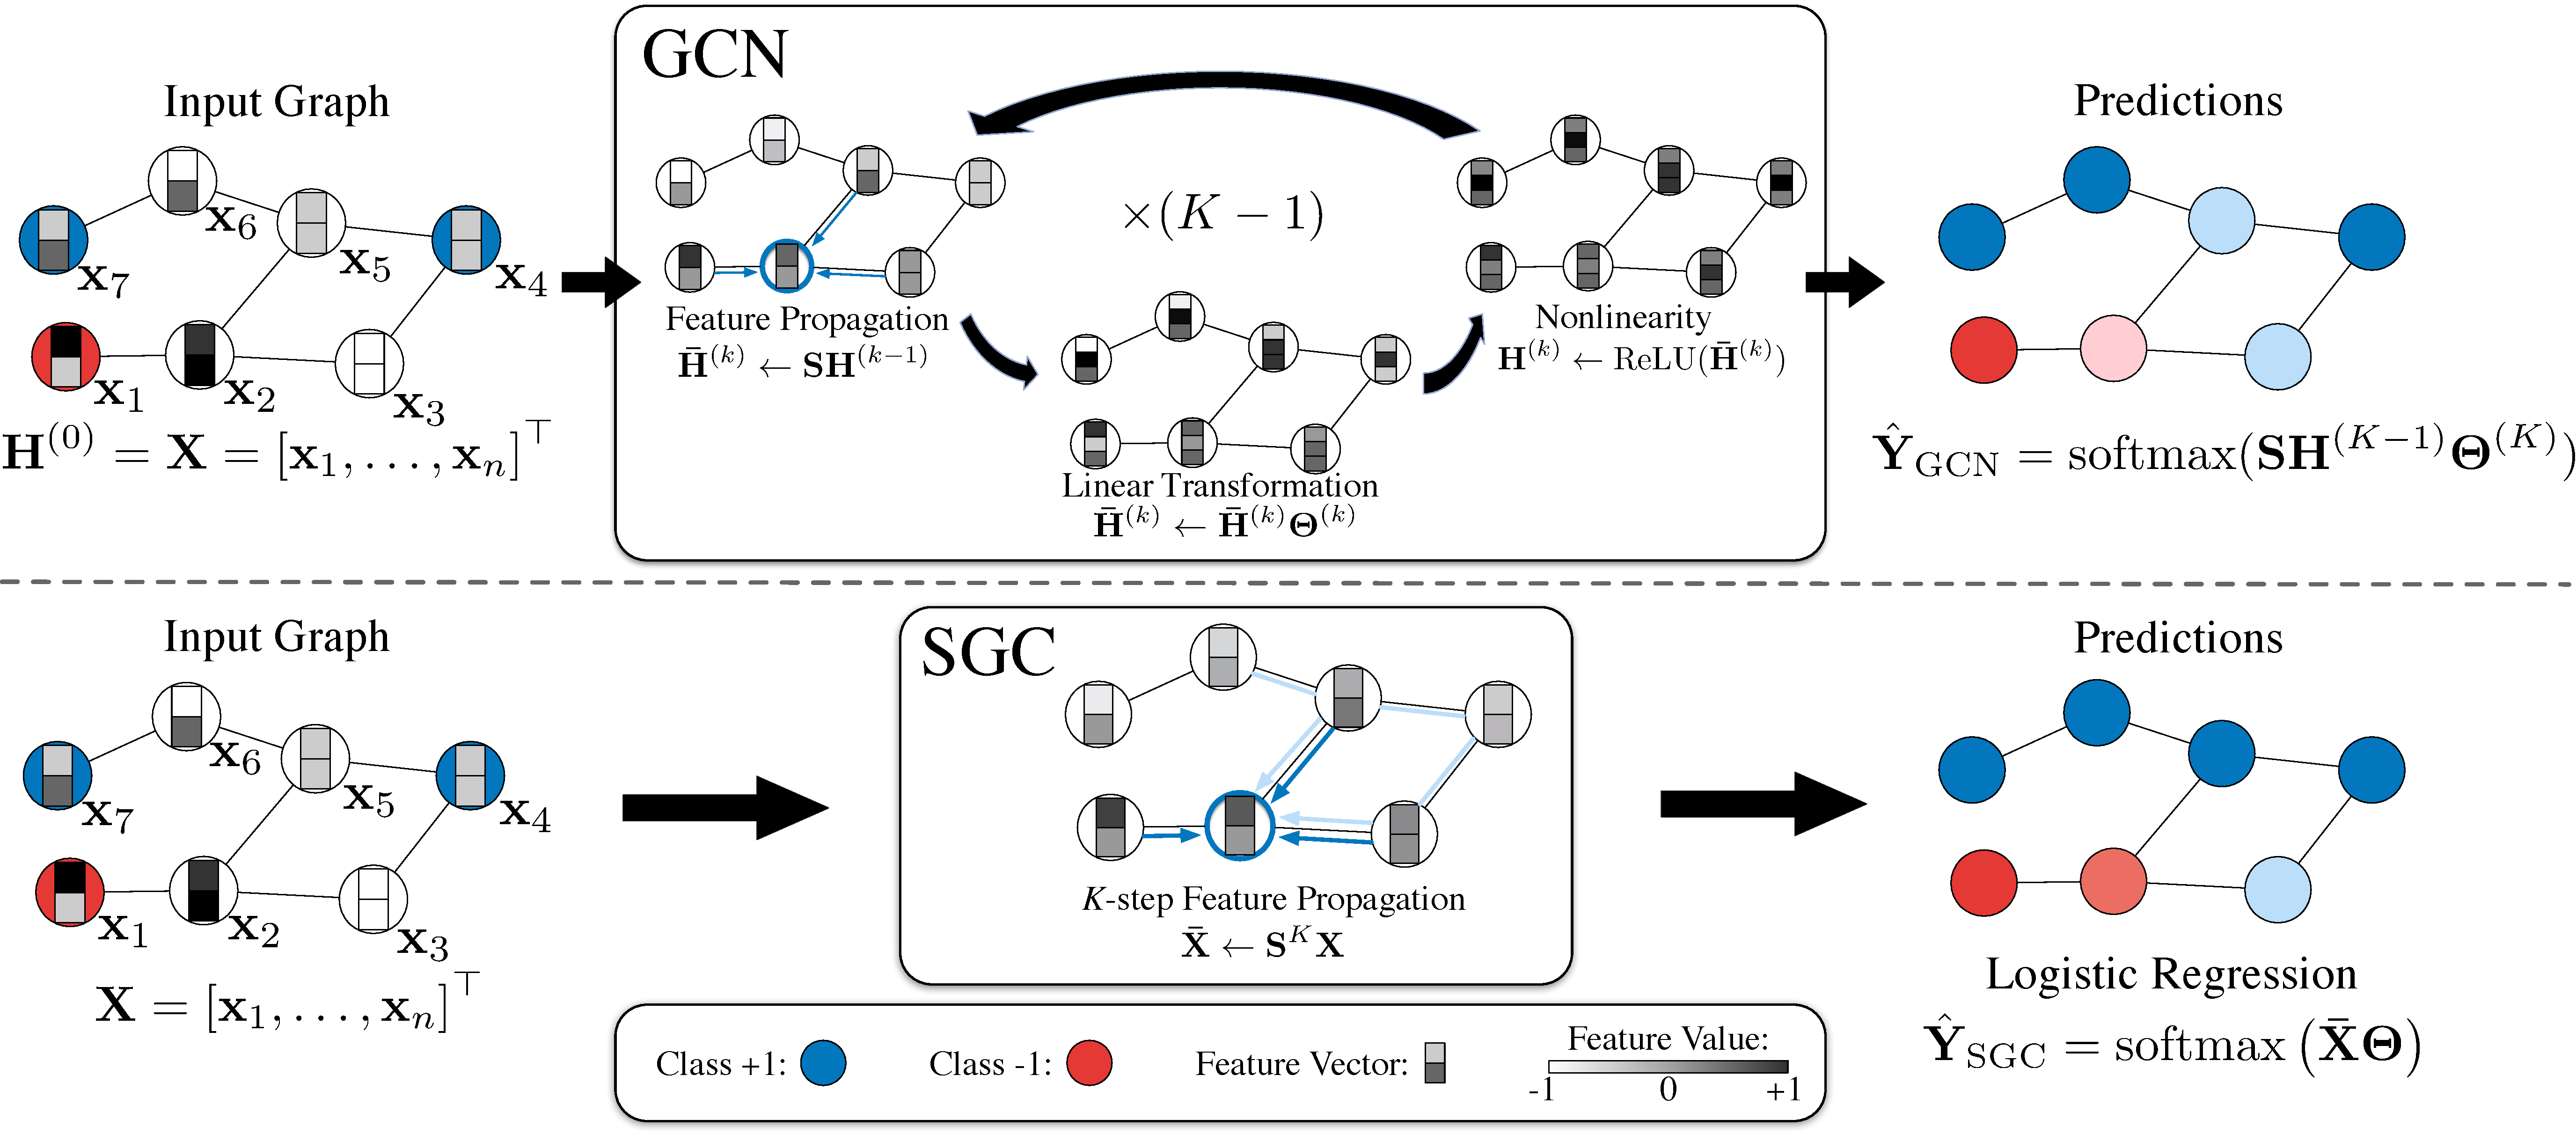
\includegraphics[width=1.0\linewidth]{figures/gcn5.pdf}
    \caption{Schematic layout of a GCN v.s. a SGC. \textit{Top row:} The GCN  transforms the feature vectors repeatedly throughout $K$ layers and then applies a linear classifier on the final representation. \textit{Bottom row:}  the \method{} reduces the entire procedure to a simple feature propagation step followed by standard logistic regression. }
    \label{fig:method}
\end{figure*}

However, possibly because GCNs were proposed after the recent ``renaissance" of neural networks, they tend to be a rare exception to this trend. GCNs are built upon multi-layer neural networks, and were never an extension of a simpler (insufficient) linear counterpart. 

In this paper, we observe that GCNs inherit considerable  complexity from their deep learning lineage, which can be burdensome and unnecessary for less demanding applications. Motivated by the glaring historic omission of a simpler predecessor, we aim to derive the simplest linear model that ``could have'' preceded the GCN, had a more ``traditional'' path been taken. We reduce the excess complexity of GCNs by repeatedly removing the nonlinearities between GCN layers and collapsing the resulting function into a single linear transformation. We empirically show that the final linear model exhibits comparable or even superior performance to GCNs on a variety of tasks while being computationally more efficient and fitting significantly fewer parameters. We refer to this simplified linear model as \Method{} (\method{}). 

In contrast to its nonlinear counterparts, the  \method{} is intuitively interpretable and 
we provide a theoretical analysis from the graph convolution perspective. 
Notably, feature extraction in \method{} corresponds to a single fixed filter applied to each feature dimension. 
\citet{gcn} empirically observe that the ``renormalization trick", i.e. adding self-loops to the graph, improves accuracy, and we demonstrate that this method effectively shrinks the graph spectral domain, resulting in a low-pass-type filter when applied to \method{}. 
Crucially, this filtering operation gives rise to locally smooth features across the graph~\cite{Bruna13}.

Through an empirical assessment on node classification benchmark datasets for citation and social networks, we show that the \method{} achieves comparable performance to GCN and other state-of-the-art graph neural networks. However, it is significantly faster, and even outperforms  FastGCN~\citep{FastGCN} by  up to two orders of magnitude on the largest dataset (Reddit) in our evaluation. 
Finally, we demonstrate that \method{} extrapolates its effectiveness to a wide-range of downstream tasks. In particular, \method{} rivals, if not surpasses, GCN-based approaches on text classification, user geolocation, relation extraction, and zero-shot image classification tasks. 
The code is available on Github\footnote{\url{https://github.com/Tiiiger/SGC}}.

